%%%%%%%%%%%%%%%%%%%%%%%%%%%%%%%%%%%%%%%%%%%%%%%%%%%%%%%%%%%%%%%%%%%%%%%%%%
%   This is frontpage.tex file needed for the dmathesis.cls file.  You   %
%  have to  put this file in the same directory with your thesis files.  %
%                Written by M. Imran 2001/06/18                          % 
%                 No Copyright for this file                             % 
%                 Save your time and enjoy it                            % 
%                                                                        % 
%%%%%%%%%%%%%%%%%%%%%%%%%%%%%%%%%%%%%%%%%%%%%%%%%%%%%%%%%%%%%%%%%%%%%%%%%%%
%%%%%%%%%%%%%%%%%%%%%%%%%%%%%%%%%%%%%%%%%%%%%%%%%%%%%%%%%%%%%%%%%%%%%%%%%%%
%%%%%%%%%%%%%%%%           The title page           %%%%%%%%%%%%%%%%%%%%%%%  
%%%%%%%%%%%%%%%%%%%%%%%%%%%%%%%%%%%%%%%%%%%%%%%%%%%%%%%%%%%%%%%%%%%%%%%%%%%
\pagenumbering{roman}
%\pagenumbering{arabic}

\setcounter{page}{1}

\newpage

\thispagestyle{empty}
\begin{center}
{\Huge \bf Flexible Univariate Extreme Value Modelling with Applications in Insurance\par}
 
  \vspace*{1cm}
  
  {\large\bf Gaonyalelwe Maribe\\(2007052190)}\\
  
 \vspace*{2cm}
 
\textbf{Promoters:}\\
Dr. Andrehette Verster \& Prof. Jan Beirlant

  \vfill

  {\Large A Thesis submitted in fulfillment of the degree of\\
         [1mm] Doctor of Philosophy}
  \vspace*{0.4cm}
  
  % Put your university logo here if you wish.
   \begin{center}
   
\includegraphics[width=7cm]{UFS.pdf}
   \end{center}

  {\large UNIVERSITY OF THE FREE STATE\\
          [-3mm] Faculty of Natural and Agricultural Sciences\\
          [-3mm] Department of Mathematical Statistics and Actuarial Science\\
          [1mm]  December 2018}

\end{center}

%%%%%%%%%%%%%%%%%%%%%%%%%%%%%%%%%%%%%%%%%%%%%%%%%%%%%%%%%%%%%%%%%%%%%%%%%%%
%%%%%%%%%%%%%%%% The dedication page, of you have one  %%%%%%%%%%%%%%%%%%%%  
%%%%%%%%%%%%%%%%%%%%%%%%%%%%%%%%%%%%%%%%%%%%%%%%%%%%%%%%%%%%%%%%%%%%%%%%%%%
\newpage
\thispagestyle{empty}
\begin{center}
 \vspace*{6cm}
\textit{\LARGE {In dedication to a dream deferred}}\\
\begin{minipage}{30em}
\vspace*{1cm}
\begin{center}
{\it
What happens to a dream deferred?
\\
Does it dry up\\
like a raisin in the sun?\\
Or fester like a sore—\\
And then run?\\
Does it stink like rotten meat?\\
Or crust and sugar over—\\
like a syrupy sweet?
\\
Maybe it just sags
like a heavy load.
\\
Or does it explode?\\
---\textbf{by Langston Hughes}
 }
  \end{center}
\end{minipage}
 \end{center}

%%%%%%%%%%%%%%%%%%%%%%%%%%%%%%%%%%%%%%%%%%%%%%%%%%%%%%%%%%%%%%%%%%%%%%%%%%%
%%%%%%%%%%%%%%%%%%           The abstract page         %%%%%%%%%%%%%%%%%%%%  
%%%%%%%%%%%%%%%%%%%%%%%%%%%%%%%%%%%%%%%%%%%%%%%%%%%%%%%%%%%%%%%%%%%%%%%%%%%
\newpage
\thispagestyle{empty}
\addcontentsline{toc}{chapter}{\numberline{}Abstract}
\begin{center}
 {\Large \bf Flexible Univariate Extreme Value Modelling with Applications in Insurance}\\
  \vspace*{1cm}
  \textbf{\large Gaonyalelwe Maribe\\(2007052190)}\\
  \vspace*{0.5cm}
  {\large Submitted for the degree of Doctor of Philosophy\\ December 2018}

  \vspace*{1cm}
  \textbf{\large Abstract}\\
    
\end{center}
Bias reduction in tail estimation has received considerable interest in extreme value analysis. Estimation methods that minimise the bias while keeping the mean squared error (MSE) under control, are especially useful when applying classical methods such as the \cite{hill1975simple} estimator. In the case of heavy tailed distributions, \cite{caeiro2005direct} proposed minimum variance reduced bias estimators of the extreme value index, where the bias is reduced without increasing the variance with respect to the Hill estimator. This method is based on adequate external estimation of a pair of parameters of second order slow variation under a third order condition. 
\\\\
In this thesis we revisit this problem and exploit the mathematical fact that the bias of the Hill estimator tends to zero as the threshold increases. This leads to a shrinkage estimation of the extreme value index, which allows for a penalised likelihood and a Bayesian implementation of the extended Pareto distribution, as developed in \cite{beirlant2009second}. Asymptotic results for the resulting shrinkage penalised likelihood estimator of the extreme value index are presented. Finite sample simulation results are proposed both for the penalised likelihood and Bayesian implementation. We then compare with the minimum variance reduced bias estimators of \cite{caeiro2005direct}.
\\\\
The subject of tail estimation for randomly censored data from a heavy tailed distribution has received growing attention, motivated by applications for instance in actuarial statistics. The bias of the available estimators of the extreme value index can be substantial and depends strongly on the amount of censoring. We review the available estimators, propose a bias reduced estimator, and show again how shrinkage estimation can help to keep the MSE under control. A bootstrap algorithm is proposed to construct confidence intervals. These new proposals are compared with the existing estimators through simulation results. A detailed study of a long-tailed car insurance portfolio is made, which typically exhibit heavy censoring.
\\\\
In recent years, several attempts have been made to extend tail modelling towards the modal part of the data. Great efforts have been made in the development of extreme value models which allow for simultaneous estimation of the threshold, quantification of threshold uncertainties and inference based on all the data. 
\\
When fitting second order models it turns out that the bias of the resulting extreme value estimators is significantly reduced compared to the classical tail fits using only the first order tail component based on the Pareto or generalised Pareto (GP) fits to peaks over threshold (POT) distributions. 
\\
This thesis proposes a novel bias reduced tail fitting technique, improving upon the classical GP approximation for POT using the flexible semiparametric GP modelling introduced in Tencaliec et al. (2018). We also revisit and extend the second order refined POT approach started in \cite{beirlant2009second} to all max-domains of attraction using flexible semiparametric modelling of the second order component. In this way we relax the classical second order regular variation assumptions.

%%%%%%%%%%%%%%%%%%%%%%%%%%%%%%%%%%%%%%%%%%%%%%%%%%%%%%%%%%%%%%%%%%%%%%%%%%%
%%%%%%%%%%%%%%%%%%          The declaration page         %%%%%%%%%%%%%%%%%%  
%%%%%%%%%%%%%%%%%%%%%%%%%%%%%%%%%%%%%%%%%%%%%%%%%%%%%%%%%%%%%%%%%%%%%%%%%%%
\newpage
\chapter*{Declaration}
\thispagestyle{empty}
\addcontentsline{toc}{chapter}{\numberline{}Declaration}
I, Gaonyalelwe Maribe, hereby declare that this work, submitted for the degree Ph.D (Mathematical Statistics) at the University of the Free State is my own original work, and has not been submitted at another university/faculty for any reward, recognition, or degree. I further declare that all sources cited or quoted are indicated and acknowledged by means of a comprehensive list of references. Copyright hereby cedes to the University of the Free State.
	\vspace{0.1in}
	%\hrule
	\begin{figure}[!h]
		\centering
		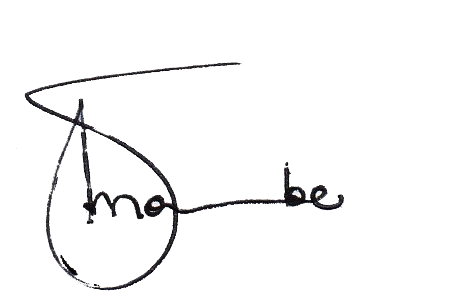
\includegraphics[viewport = 0 107 350 50,width=12cm]{./plots/signature.png}
	\end{figure}  

	\vspace {0.6in}
	\textbf{Signature}:\makebox[1.9in]{\hrulefill} \hspace{1.3in}\textbf{Date: \today} \\
\newpage
%%%%%%%%%%%%%%%%%%%%%%%%%%%%%%%%%%%%%%%%%%%%%%%%%%%%%%%%%%%%%%%%%%%%%%%%%%%
%%%%%%%%%%%%%%%%%%     The acknowledgements page         %%%%%%%%%%%%%%%%%%  
%%%%%%%%%%%%%%%%%%%%%%%%%%%%%%%%%%%%%%%%%%%%%%%%%%%%%%%%%%%%%%%%%%%%%%%%%%%
%\chapter*{Research output}
%\thispagestyle{empty}
%\addcontentsline{toc}{chapter}{\numberline{}Acknowledgements} 
%This thesis is based on three manuscripts:

%\begin{table}[h]
%\resizebox{\textwidth}{!}{%
%\begin{tabular}{@{}ll@{}}
%\toprule
%\textbf{Manuscript}                                                                                              %                                                                                                                 %                             & \textbf{Publication outcome}                                                      %                                             \\ \midrule
%\multicolumn{1}{|l|}{\textit{\begin{tabular}[c]{@{}l@{}}1. Using shrinkage estimators to reduce bias\\  and MSE %in estimation of heavy tails \\ (Beirlant, J., Maribe, G. and Verster, A., 2017)\end{tabular}}}                  %%                             & \multicolumn{1}{l|}{Accepted (fourthcoming) by REVSTAT}                          %                                              \\ \midrule
%\multicolumn{1}{|l|}{\textit{\begin{tabular}[c]{@{}l@{}}2. Penalised bias reduction in extreme value \\ %estimation for censored Pareto-type data, \\ and long-tailed insurance applications \\ (Beirlant, J., Maribe, G. %and Verster, A., 2018)\end{tabular}}} & \multicolumn{1}{l|}{\begin{tabular}[c]{@{}l@{}}Accepted and published by %\\ Insurance: Mathematics and Economics\end{tabular}} \\ \midrule
%\multicolumn{1}{|l|}{\textit{\begin{tabular}[c]{@{}l@{}}3. Bias Reduced Peaks over Threshold Tail Estimation\\ %(Beirlant, J., Maribe, G., Ph. Naveau and Verster, A., 2018)\end{tabular}}}                                      %                               & \multicolumn{1}{l|}{\begin{tabular}[c]{@{}l@{}}Submitted to \\ Computational %Statistics \& Data Analysis\end{tabular}}         \\ \bottomrule
%\end{tabular}%
%}
%\end{table}
%\newpage
%%%%%%%%%%%%%%%%%%%%%%%%%%%%%%%%%%%%%%%%%%%%%%%%%%%%%%%%%%%%%%%%%%%%%%%%%%%
%%%%%%%%%%%%%%%%%%     The acknowledgements page         %%%%%%%%%%%%%%%%%%  
%%%%%%%%%%%%%%%%%%%%%%%%%%%%%%%%%%%%%%%%%%%%%%%%%%%%%%%%%%%%%%%%%%%%%%%%%%%
\chapter*{Acknowledgements}
\thispagestyle{empty}
\addcontentsline{toc}{chapter}{\numberline{}Acknowledgements} 
I would firstly like to thank \textbf{God} for all the blessings he has showered upon me and my family, for the daily strength he has given me and for all the people he has placed in my path to make life more meaningful.
\\\\
To my family for all the sacrifices they had to make for my education. Again to my family and friends for being understanding and having to deal with my ``research moods", most especially \textbf{Kgabo Mphahlele}.
\\\\
Towards the end of the term in November of 2014, I found myself in \textbf{Andréhette Verster's} office, seeking mentorship for my Honours research project. Not knowing she would continue to mentor me throughout my masters and PhD studies. This visit to her office has been one of the most fruitful endeavours of my life. I am truly grateful to have been called your student.
\\\\
To \textbf{Jan Beirlant} from {\it KU Leuven, Belgium}, a great teacher and mentor. From you, I have learned a lot about myself. I would like to thank you for taking out your time to work with me. I jokingly like to refer to you as my grandfather \smiley{}, this is because no one has ever had so much patience in explaining difficult concepts to me as you have. I am truly grateful for the life long contribution you have made in my life.
\\\\
To \textbf{Philippe Naveau} from \textit{Laboratoire des Sciences du Climat et de l'Environnement, CNRS, Université Paris-Saclay}, thank you for our collaborative work described in Chapter 5, and for being a fantastic host on our visit to Paris.
\\\\
I would also like to take pleasure in thanking \textbf{Sean van der Merwe} for his valuable advice concerning the Bayesian implementations in Chapter 3.
\\\\
A special thanks goes out to \textbf{Rym and Julien Worms} for their helpful discussions and suggestions on the topic of tail estimation for randomly censored data. 
\\\\
I would also like to thank and acknowledge the UFS High-Performance Computing (HPC) unit for providing me with the massive amount of computing resources I used to conduct simulation studies. More especially \textbf{Stephanus Riekert}, I am truly grateful for all the technical support you provided me.
\\\\
Thanks to the REVSTAT as well as Insurance: Mathematics \& Economics referees for their constructive comments which improved the presentation of the accepted papers significantly. I extend this thanks to the assessors taking out their invaluable time to asses this PhD thesis.
\\\\
I would lastly like to thank the ``\textit{SASA‐NRF GRANT: Academic statistics bursary fund}" for sponsoring this PhD research.

\textit{This work is based on the research supported wholly/in part by the National Research Foundation of South Africa (Grant Number 102628). The Grantholder acknowledges that opinions, findings and conclusions or recommendations expressed in any publication generated by the NRF supported research is that of the author(s), and that the NRF accepts no liability whatsoever in this regard.}\newpage
\cleardoublepage
%%%%%%%%%%%%%%%%%%%%%%%%%%%%%%%%%%%%%%%%%%%%%%%%%%%%%%%%%%%%%%%%%%%%%%%%%%%%
%%%%%%%%%%%%%%%%%%         List of acronyms              %%%%%%%%%%%%%%%%%%  
%%%%%%%%%%%%%%%%%%%%%%%%%%%%%%%%%%%%%%%%%%%%%%%%%%%%%%%%%%%%%%%%%%%%%%%%%%%
\chapter*{List of acronyms}
\thispagestyle{empty}
\addcontentsline{toc}{chapter}{\numberline{}List of acronyms}
\begin{tabular}{p{3cm}p{8cm}}
\textbf{2ERV} & Second order extended regular variation\\
\textbf{CH} & Corrected Hill \\
\textbf{CLT} & Central limit theorem\\
\textbf{CDF} & Cumulative distribution function\\
\textbf{IID} & Independent, identically distributed\\
\textbf{EP}  & Extended Pareto\\
\textbf{EPD}  & Extended Pareto distribution \\
\textbf{ERV} & Extended regular variation\\
\textbf{EVI} & Extreme value index\\
\textbf{EVT} & Extreme value theory\\
\textbf{GEV} & Generalised extreme value\\
\textbf{GP} & Generalised Pareto\\
\textbf{GPD} & Generalised Pareto distribution\\
\textbf{HTE} & Heavier than exponential\\
\textbf{KM} & Kaplan-Meier\\ 
\textbf{LTE} & Lighter than exponential\\
\textbf{ML} & Maximum likelihood\\
\textbf{MLE} & Maximum likelihood estimate\\
\textbf{MVBR} & Minimum variance reduced bias\\
\textbf{PML} & Penalised maximum likelihood\\
\textbf{POT} & Peaks over threshold\\
\end{tabular}
\clearpage
\cleardoublepage

%%%%%%%%%%%%%%%%%%%%%%%%%%%%%%%%%%%%%%%%%%%%%%%%%%%%%%%%%%%%%%%%%%%%%%%%%%%
%%%%%%%%%%%%%%%%%%         Mathematical notations        %%%%%%%%%%%%%%%%%%  
%%%%%%%%%%%%%%%%%%%%%%%%%%%%%%%%%%%%%%%%%%%%%%%%%%%%%%%%%%%%%%%%%%%%%%%%%%%
\chapter*{Mathematical notation}
\thispagestyle{empty}
\addcontentsline{toc}{chapter}{\numberline{}Mathematical notation}
\begin{tabular}{p{4cm}p{12cm}}
$\gamma$ & Extreme value index.\\
$\mathcal{D}(G_{\gamma})$ & Domain of attraction of $G_{\gamma}$.\\
$\mathcal{F}$ & Class of distributions in the Fréchet domain of attraction.\\
$F^{\leftarrow}$ &	left continuous inverse of the distribution function $F$.\\
$f\in RV_{\rho}$ & $f$ is regular varying with index $\rho$.\\
$\Delta$ & Censoring indicator, 0 if the observation is right-censored and 1 if not.\\
$\l_{pen}$ & Penalised likelihood.\\
$\blacktriangle$ & Indicates the end of a definition, proof, lemma or proposition.\\
$\ell_{a}, \ell_{\delta}, \ell_U$ \& $\ell_U$ & Slowly varying functions.\\
$f\in 2ERV_{\gamma,\rho}$ &  $f$ is of second order extended regular variation.\\
$Q(p)$ & The quantile function denoted by $Q(p)=\inf\{x|F(x)\geq p\}$.\\
$H_{k,n}$ & The Hill estimator based on $k$ excesses above the threshold.\\
$t\uparrow \infty$ & $t$ approaches $\infty$ from below, in an increasing manner.\\
$\to^d \mathcal{N}_p$ & Converges in distribution to a $p$ dimensional Normal.\\
$\omega$ & Tuning constant regulating the amount of penalty.\\
$E_{\infty},\ Var_{\infty}\ \ \&\ MSE_{\infty}$ & Asymptotic bias, variance and mean squared error.\\
${\cal T}$ and ${\cal E}$ & Transformed and extended models.
\end{tabular}
\cleardoublepage
%%%%%%%%%%%%%%%%%%%%%%%%%%%%%%%%%%%%%%%%%%%%%%%%%%%%%%%%%%%%%%%%%%%%%%%%%%%
%%%%%%%%    tableofcontents, listoffigures and listoftables       %%%%%%%%%
%%%%%%%%        Command if you do not have  them                  %%%%%%%%%
%%%%%%%%%%%%%%%%%%%%%%%%%%%%%%%%%%%%%%%%%%%%%%%%%%%%%%%%%%%%%%%%%%%%%%%%%%%
\tableofcontents
\newpage
\listoffigures
\newpage
\listoftables
\newpage
\clearpage

\newpage
%%%%%%%%%%%%%%%%%%%%%%%%%%%%%%%%%%%%%%%%%%%%%%%%%%%%%%%%%%%%%%%%%%%%%%%%%%%
%%%%%%%%%%%%%%%%%%%%%%   END OF FRONT PAGE %%%%%%%%%%%%%%%%%%%%%%%%%%%%%%%%
%%%%%%%%%%%%%%%%%%%%%%%%%%%%%%%%%%%%%%%%%%%%%%%%%%%%%%%%%%%%%%%%%%%%%%%%%%%
